% =====================================================================
% RegCheck — NeurIPS 2026 Workshop on AI for Meta-Science (position track, 8pp)
% Rewrite of arXiv:2601.13330v2. Text provenance is marked throughout:
%   [VERBATIM]    — unchanged from v2
%   [COMPRESSED]  — v2 text with sentences cut, surviving text unchanged
%   [NEW]         — new prose for this version
% Deadline: 29 August 2026 (AoE). Submissions via OpenReview.
% TODO(jamie): check the workshop's OpenReview page for anonymity policy.
%   A deployed, named tool cannot be meaningfully anonymised; if double-blind,
%   email the organisers. If anonymous submission is required, switch to
%   \usepackage{neurips_2026} (no option) and strip the URLs/self-citations.
% TODO(jamie): references.bib needs entries for the NEW keys listed at the
%   bibliography at the end of this file.
% =====================================================================
\documentclass{article}

% The CFP asks for the NeurIPS 2026 LaTeX template with the footnote changed.
\usepackage[final]{neurips_2026}
\makeatletter
\renewcommand{\@noticestring}{Submitted to AI for Meta-Science workshop (NeurIPS 2026)}
\makeatother

\usepackage[utf8]{inputenc}
\usepackage[T1]{fontenc}
\usepackage{hyperref}
\usepackage{url}
\usepackage{booktabs}
\usepackage{graphicx}
\usepackage{array}
\usepackage{microtype}
\usepackage[nameinlink]{cleveref}
\usepackage{natbib}
\bibliographystyle{plainnat}

% Alternative titles considered:
%   RegCheck: Verifiable, Structured Comparison of Study Registrations and Papers
%   RegCheck: A Scoped Verifier for Registration--Paper Consistency, Not an AI Reviewer
\title{RegCheck: Registration--Paper Consistency Checking\\as Peer-Review Infrastructure}

\author{%
  Jamie Cummins\thanks{Corresponding author: \texttt{jamie.cummins@unibe.ch}} \\
  Institute of Psychology, University of Bern\\
  Bennett Institute of Applied Data Science, University of Oxford
  \And
  Beth Clarke \\
  Institute of Psychology, University of Bern
  \And
  Ian Hussey \\
  Institute of Psychology, University of Bern
  \And
  Malte Elson \\
  Institute of Psychology, University of Bern
}

\begin{document}

\maketitle

% ---------------------------------------------------------------------
\begin{abstract} % [NEW] (reuses phrases from the v2 abstract)
Across the social and medical sciences, researchers recognise that specifying
planned research activities in advance (i.e., ``registration'') has benefits for
both the transparency and rigour of science. Yet registrations deliver these
benefits only if they are checked against the papers they accompany, and in
practice this checking rarely happens: it is labour- and time-intensive, and
peer reviewers seldom do it. We present RegCheck
(\url{https://regcheck.app}), an open-source, modular, LLM-assisted tool for
structured registration--paper comparison, and the general architecture behind
it: \emph{Parity}, organised by the four-step \emph{IDEA} framework (Ingest,
Define, Extract, Adjudicate), which separates document parsing, human-defined
comparison dimensions, evidence retrieval, and model adjudication into
independently evaluable stages, and confines generative models to the final
step. We argue that ad hoc use of commercial chat models cannot support
standardised, reproducible, verifiable, or confidential research evaluation, and
that the load-bearing design problem for tools of this class is the
specification of the comparison---its dimensions and verdict semantics---rather
than model capability. Every judgement RegCheck renders is a per-dimension
verdict (deviation, no deviation, or insufficient evidence) supported by
verbatim, click-through quotations from both documents, so that users
verify---rather than defer to---its judgements. In a companion validation on 62
clinical trials previously audited by the COMPare project, a RegCheck-based
workflow agreed with expert audits on 85.6\% of misreporting judgements (94.8\%
after adjudication of discrepancies) at a cost of \$5.94 per paper. RegCheck is
free to use, open source, and can be run fully locally.
\end{abstract}

% ---------------------------------------------------------------------
\section{Introduction}\label{sec:intro}

% [VERBATIM] v2 §1 ¶1
The importance of registering study designs, materials, hypotheses, outcomes,
and processing/analysis plans for the transparency and rigour of research has
seen increasing recognition in the medical and social sciences in the last 20
years. In clinical trials, registration is a legal requirement according to the
regulations governing many countries such as the United States
\citep{noauthor_nih_nodate} and Europe \citep{noauthor_regulation_2014}. Even
when not legally required, registration sees use across the sciences. In general
medical research, the creation of registrations (or publication of study
protocols) is growing in prevalence \citep{tan_prevalence_2019}; the same trend
can also be seen in economics, with pre-analysis plans
\citep{ofosu_pre-analysis_2023}, and in psychology, with preregistration (and
more recently, Registered Reports; \citealp{chambers_past_2021,
hardwicke_prevalence_2024}). Although different fields have different labels,
norms, and literatures discussing these approaches, for the sake of consistency
here, we refer to all of these using the term ``registration''.

% [COMPRESSED] v2 §1 ¶2 (last sentence cut) + ¶3 (Lakens framing sentence cut)
In principle, these registrations improve the transparency of decision making
and plans associated with research programs. Crucially, registrations enable the
reader to distinguish which analytic decisions were made before and after
observing the data, which can have implications for the veracity and severity of
the reported statistical tests \citep{kaplan_likelihood_2015}, and allow readers
to assess the risk of bias and calibrate their confidence in the results
accordingly \citep{hardwicke_reducing_2023}. In practice, however, study
registration is often more complex. Researchers may need to deviate from their
registration for a variety of reasons, and although some deviations could be
unproblematic or trivial, others can seriously impact the severity of the
test(s) of the predictions \citep{lakens_when_2024}. This is far from a distant
concern---several meta-science studies across a variety of fields have found
that deviations from registrations are common \citep{bakker_ensuring_2020,
claesen_comparing_2021, goldacre_compare_2019, hahn_cross-sectional_2025,
heirene_preregistration_2024, li_systematic_2018, ofosu_pre-analysis_2023,
poole_systematic_2025, targ_meta-research_group__collaborators_estimating_2023,
van_den_akker_selective_2023, van_den_akker_potential_2024}, and that these
deviations are often not disclosed in the final paper
\citep{targ_meta-research_group__collaborators_estimating_2023,
van_den_akker_selective_2023, van_den_akker_potential_2024}\footnote{Another
serious issue is that registrations are often underspecified and do not provide
sufficient details to deviate from to begin with \citep{bakker_ensuring_2020,
hahn_cross-sectional_2025, ofosu_pre-analysis_2023, poole_systematic_2025,
van_den_akker_potential_2024}.}.

% [VERBATIM] v2 §1 ¶4–¶5 (merged; "This may also serve to explain..." retained)
So how do these undisclosed deviations make it past peer review? The answer is
probably quite simple. Checking registrations against the eventually published
paper is a time-intensive and laborious process. Given peer reviewers are
already overburdened \citep{adam_peer-review_2025}, the fairly substantial
additional task of checking studies against their registrations seems unlikely
to be done. Indeed, one study of articles published at \emph{PLOS} suggests that
very few editors and reviewers engage with registrations during the peer review
process \citep[see also][]{syed_data_2025, spitzer_registered_2023}. In a survey
of reviewers for medical journals, only 34.3\% indicated they had examined the
information on a trial registry within the past two years
\citep{mathieu_use_2013}. This may also serve to explain why deviations are not
reported by authors themselves: at least in some cases, it is plausible that
authors are unaware of such deviations, given that checking for them is
laborious. If registrations are never examined or evaluated, then we might be
simply assuming that the risk of bias has been reduced when this may not be the
case at all.

% [VERBATIM] v2 §1 ¶6–¶7 (lightly trimmed at the join)
The recent advent of generative large language models (LLMs) offers the
possibility of automating portions of the work involved in registration--paper
comparisons, assisting reviewers in a task that they seem to avoid (note that we
refer to ``registration--paper'' comparisons throughout, but of course such
processes can be done with drafts of manuscripts prior to publication or
submission to a journal). Indeed, the simplest form of this automation is
already accessible to the average researcher: upload both documents to a
commercial LLM and prompt it to compare them. As we argue in
\cref{sec:why-not-llm}, however, this ad hoc approach cannot support robust
research evaluation. What is needed instead is an approach which ensures
consistency and standardisation in prompt content, comparison logic, and output
across calls and users, while also ensuring that expert knowledge is applied by
(i) allowing researchers to specify which dimensions should be examined, and
(ii) facilitating researchers' assessment of discrepancies. To meet these needs,
we have developed RegCheck: a tool which automatically extracts the most
relevant text from registrations and papers, easily facilitating comparison
between these sources. It provides a pipeline that parses registration and
publication texts, lets users specify what dimensions they want to check, and
produces structured, auditable reports which are shareable via unique links. By
lowering the difficulty barrier for checking registrations without removing
expert oversight, RegCheck aims to make consistency checks a routine part of
scientific workflows.

% [NEW] related tools positioning (short; adapted from earlier editorial draft)
RegCheck joins a small but growing set of tools bringing computational
assistance to research integrity. Statistical-consistency checkers such as
statcheck and GRIM verify the internal numerical consistency of reported
results; reporting-checkers assess whether papers report key methodological
criteria; and checklists such as INSPECT-SR help reviewers identify potentially
problematic trials during systematic-review screening
\citep{wilkinson_inspect-sr_2025}. RegCheck is complementary to these: rather
than checking a paper against internal consistency or general reporting
standards, it checks a paper against \emph{its own study's registration}, along
dimensions the user defines.

% [NEW] thesis + reference-description sentence + contributions
% (first two sentences [VERBATIM] from v2 §1 ¶8)
RegCheck is a single instance of a broader class of emerging meta-scientific
tools: those whose purpose is to provide (semi-)automated comparisons between
academic research objects for which consistency is expected and deviations are
informative. We refer to the abstract architecture underlying this class as
\emph{Parity}. The position this paper takes is that, for tools of this class,
the load-bearing design problem is \emph{specification rather than model
capability}: deciding what is compared, by whom, and under what verdict
semantics matters more---and is harder---than the model call that renders any
single judgement. A tool built this way assists peer review without becoming an
``AI reviewer'': every judgement it produces is scoped, human-specified, and
verifiable. This paper serves as the reference description of RegCheck, and
makes five contributions:
\begin{enumerate}
  \item \textbf{Parity and the IDEA framework} (\cref{sec:parity}): a structured
  decomposition of meta-scientific consistency checking into ingestion,
  human-led definition, evidence extraction, and adjudication, applicable well
  beyond registration--paper comparison.
  \item \textbf{Why not just ask an LLM} (\cref{sec:why-not-llm}): six reasons
  ad hoc LLM use cannot support robust research evaluation---each of which, we
  show, is addressed by a specific IDEA stage rather than by a better model.
  \item \textbf{Dimensions as the unit of comparison} (\cref{sec:dimensions}): a
  formulation of registration--paper comparison in which the basis of comparison
  is human-defined, each dimension is adjudicated independently, and verdicts
  are three-valued, with \emph{insufficient evidence} as a first-class outcome.
  \item \textbf{A worked example} (\cref{sec:worked-example}): a complete
  hypothetical report illustrating the verdict semantics and the verification
  affordances of the report interface.
  \item \textbf{RegCheck itself} (\cref{sec:regcheck,sec:validation}): a
  deployed, free, open-source instance of Parity, externally validated against
  expert audits of clinical trials \citep{cummins_automating_2026}.
\end{enumerate}

% ---------------------------------------------------------------------
\section{Why Not Just Ask an LLM?}\label{sec:why-not-llm}

% [VERBATIM] v2 §2 opening
Before describing the workflow itself, it is worth engaging with a simple
question: since generative LLMs are already widely accessible, why is a
dedicated tool needed at all? Any researcher can already upload a registration
and a paper to a commercial chat model and prompt it to compare them; in one
sense, the automation problem is ``solved''. However, such an ad hoc approach
cannot support comparisons that are standardised, reproducible, verifiable, and
confidential---all properties that formal research evaluation demands. Below we
discuss six problems associated with simply using a standard LLM chat interface.

\begin{enumerate}
  % [COMPRESSED] v2 §2 item 1 (two mid-list sentences cut)
  \item \textbf{Analytic flexibility.} Even for an identical underlying task,
  LLM output can vary substantially with the phrasing of the prompt, the
  formatting of the documents, and the model's input parameters. For instance,
  the difference between the presence or absence of a colon in a required output
  format can shift LLMs' accuracy in a categorisation task by up to 76
  percentage points \citep{sclar_quantifying_2023}. Additionally, other analytic
  decisions (e.g., choice of values for temperature/reasoning effort, the
  granularity of prompt requests, system prompt content, and a range of other
  factors) can substantially influence the output of LLMs
  \citep{cummins_threat_2025}. This also serves as a barrier to formal
  evaluation of the performance of these tools: it is not possible to estimate
  how accurate an LLM \emph{in general} is at comparing preregistrations and
  papers, because this performance is necessarily tied to this myriad of factors
  and analytic decisions that a researcher can make (or that are obscured when
  using commercial chat interfaces, see point 2). Robust usage and evaluation
  therefore requires standardised inputs, including fixed prompt structures and
  definitions, consistent procedures for supplying source material to the model,
  and easily definable hyperparameter values.

  % [VERBATIM] v2 §2 item 2
  \item \textbf{Commercial chat interfaces are not appropriate for research
  evaluation.} In practice, ad hoc use almost always means that consumer chat
  products are used. Put simply: these interfaces are not suitable for use as a
  formal, standardised research tool. This is the case firstly because many of
  the influential analytic decisions mentioned in the previous point are
  typically gated off from the user when using commercial chat interfaces
  \citep{higgins_recommendations_2026}. Worse still, these settings are not
  merely fixed by the LLM provider, but unstable: for example, versions of the
  deployed model, system prompts, and server-side processing steps may be
  changed without notice to, or control by, users.

  % [VERBATIM] v2 §2 item 3
  \item \textbf{Data privacy.} Registration--paper comparison routinely involves
  unpublished manuscripts, including materials handled under the confidentiality
  expectations of peer review. When files are uploaded to a commercial chat
  interface, providers typically reserve the right, under default settings, to
  use this data for model training; usage agreements for data submitted via APIs
  are generally more restrictive. Moreover, commercial chat interfaces provide
  access only to their provider's own models: open-weight models (which can be
  hosted by parties with no commercial stake in the data, by institutions, or on
  fully local infrastructure) are largely inaccessible through them. A workflow
  built around chat interfaces therefore forecloses the strongest available
  privacy measures, such as running an identical comparison entirely on local
  infrastructure.

  % [COMPRESSED] v2 §2 item 4 (example sentence shortened)
  \item \textbf{Unwanted dependency among comparisons.} Because of the nature of
  the next-token prediction architecture that constitutes large language models,
  subsequent predictions for outputs (in a chat context) are influenced by
  previous predictions. Asking a model to make comparisons on multiple
  dimensions of interest in a single pass necessarily introduces dependencies
  among the resulting judgements because output is generated sequentially---for
  example, if a model states that the registration and paper do not match based
  on hypotheses (when in reality they do), then this may also increase the
  likelihood that the model states that the registration and paper do not match
  based on the statistical analyses, given that hypotheses and statistical
  analyses may often be related. Errors can therefore propagate across
  dimensions, and dimension-level accuracy can no longer be evaluated
  independently. This makes both reproducibility and meaningful evaluation
  substantially harder to achieve.

  % [VERBATIM] v2 §2 item 5
  \item \textbf{Conflation of distinct tasks.} Simply asking an LLM to make
  these comparisons delegates a number of distinct tasks to the LLM (i.e.,
  ingestion, definition of dimensions of interest, extraction, and adjudication;
  see \cref{sec:parity}). However, this comes at the cost that other tools
  (including human input) may be more appropriate for some of these steps than
  others. It also means that it is difficult to evaluate the independent
  performance of the LLM on each of these component steps, because they are
  necessarily tied to one another (in a manner similar to point 4 above).

  % [VERBATIM] v2 §2 item 6
  \item \textbf{Verifiability.} Large language models will, by and large,
  provide a response to any query that does not breach their safety
  guidelines---including in cases where the response is incorrect
  (``hallucinations''). Any LLM-based research tool therefore needs to make the
  model's claims trivially verifiable. Although some LLM products provide
  citations for some claims, this is unsystematic and not guaranteed to occur in
  every case. If researchers must go through the documents themselves to
  identify where the LLM's claims come from, this is no more efficient than
  performing the comparison manually in the first place.
\end{enumerate}

% [VERBATIM] v2 §2 closing ¶
Importantly, none of the above-mentioned problems serve as arguments against
using LLMs for registration--paper comparison in general. Rather, these
arguments highlight the need for the use of LLMs in a standardised, transparent,
and modularised workflow which clearly delineates the different steps required
for the comparison, as well as which tool should serve to perform each of those
steps. Breaking down such workflows in this manner is the goal of the IDEA
framework and its software implementation Parity, which we now discuss.
% [NEW] bridge sentence + mapping table
\Cref{tab:problems-idea} previews the mapping: each failure mode above is
neutralised by a specific structural commitment of the framework, not by a more
capable model.

% [NEW] Table: problems → IDEA answers
\begin{table}[t]
  \centering
  \caption{The six failure modes of ad hoc LLM use, and the IDEA-stage
  commitments that address them. None of the remedies depends on model
  capability.}
  \label{tab:problems-idea}
  \small
  \begin{tabular}{@{}p{0.38\linewidth}p{0.55\linewidth}@{}}
    \toprule
    \textbf{Failure mode of ad hoc use} & \textbf{Structural answer in IDEA/Parity} \\
    \midrule
    1. Analytic flexibility &
    Fixed prompt structures, definitions, and hyperparameters at every stage;
    identical inputs yield identical set-ups across users and calls. \\
    \addlinespace[2pt]
    2. Chat interfaces unsuitable &
    A standalone pipeline exposes every analytic decision (model, reasoning
    effort, chunking, retrieval depth) as an inspectable, citable parameter. \\
    \addlinespace[2pt]
    3. Data privacy &
    Provider-neutral Extract and Adjudicate stages; local embeddings and a
    locally hosted LLM allow a comparison to run with no text leaving the
    user's environment. \\
    \addlinespace[2pt]
    4. Dependency among comparisons &
    Define fixes the dimensions ex ante; Adjudicate runs each dimension in its
    own independent call, so errors cannot propagate between dimensions. \\
    \addlinespace[2pt]
    5. Conflation of distinct tasks &
    Ingestion, Definition, Extraction, and Adjudication are separate stages
    with separate tools, each independently evaluable and replaceable. \\
    \addlinespace[2pt]
    6. Verifiability &
    Extract returns verbatim, located quotations; Adjudicate must cite them;
    the report links every claim to its source text. \\
    \bottomrule
  \end{tabular}
\end{table}

% ---------------------------------------------------------------------
\section{Parity and the IDEA Framework}\label{sec:parity}

% [VERBATIM] v2 §3 ¶1, first two sentences
Parity is the more general software workflow of which RegCheck is an instance.
It is not itself a single end-user tool, but rather a generic architecture that
can be appropriated to implement different (meta-)scientific consistency-checks
in a way that keeps inputs, evidence retrieval, and judgement steps conceptually
distinct.
% [NEW] generalisation paragraph (replaces v2's single ARRIVE/PRISMA sentence)
The motivation for this abstraction is that many scientific evaluation tasks
involve checking consistency between research artefacts, and the same structure
recurs wherever one artefact makes commitments that another is expected to
honour. Registration--paper comparison, implemented in RegCheck, is one example.
A manuscript can likewise be checked against an external reporting standard
(e.g., ARRIVE, PRISMA), where the standard's items play the role of the
registration's commitments; a paper's natural-language description of its
analyses can be checked against the code that implements them, as in our second
Parity instance, \texttt{codebot} \citep{cummins_codebot_2026}; a Stage~2
Registered Report can be checked against its accepted Stage~1 protocol; and
structured extractions made for evidence synthesis can be checked against the
source papers from which they were drawn. In each case the task decomposes
identically---documents must be ingested, the dimensions of comparison must be
specified, evidence must be located, and a judgement must be rendered---and in
each case the dimensions of comparison are normative choices that belong to the
user, not to the model.

% [VERBATIM] v2 §3 ¶2 + IDEA list
Parity is organised around a four-step conceptual framework that structures how
to think about, break down, and approach (meta-)scientific comparison,
extraction, and adjudication questions between research artefacts. We refer to
this as the IDEA framework:
\begin{enumerate}
  \item \textbf{Ingestion.} Collect all documents relevant to the specific task
  at hand, and parse them in ways that maximise their utility and clarity for
  that particular task. In practice this may involve interfacing with APIs and
  handling JSON responses (e.g., on ClinicalTrials.gov), XML extraction, PDF
  parsing, document-layout models such as GROBID, reference stripping, section
  filtering, or other deterministic preprocessing needed to transform scientific
  materials into task-ready text.
  \item \textbf{Definition.} Specify along which dimensions the scientific
  materials should be evaluated, compared, or checked. This step is explicitly
  human-defined: users (who may be reviewers, editors, or the authors
  themselves) define the dimensions of interest, whether these are
  reporting-guideline items, preregistered sample-size commitments, outcomes, or
  any other target of interest to the user.
  \item \textbf{Extraction.} Represent documents and dimension definitions in a
  form that supports targeted retrieval, and then extract the most relevant
  evidence for each dimension. In practice, this is most frequently done by the
  use of semantic embeddings models, which represent semantic information
  through numeric vectors. Text extraction is then done by splitting scientific
  documents into chunks, embedding these chunks and dimension definitions
  specified in the previous step, and querying the similarity of each chunk with
  the dimension of interest.
  \item \textbf{Adjudication.} Make a judgement for the task at hand on the
  basis of the extracted evidence. This is the stage at which generative LLMs
  are most naturally used, because the system must synthesise multiple excerpts
  and render a task-specific judgement, such as whether a registration and paper
  are consistent on a given dimension.
\end{enumerate}

% [VERBATIM] v2 §3 modularity ¶ (incl. the fine-grained-validation sentences)
In addition to providing a scaffolding for researchers to think about how to
decompose their meta-scientific workflow into distinct steps, the IDEA framework
also helpfully clarifies that different steps in the framework involve different
tools or sources of input. This also modularises the backend code, increasing
its reusability in other open-source scientific projects and allowing individual
elements of the Parity workflow to be replaced as better solutions emerge (e.g.,
for the pernicious problem of text extraction from PDFs, with which many
scientific software projects contend). This separation of the four steps, both
conceptually and in code, also enables more fine-grained validation of any given
Parity implementation: the validation of LLM-based Adjudication is distinct from
the generic difficulties of Ingestion (such as PDF text extraction), and
validation metrics can be designed to identify which steps succeed or fail.

% [VERBATIM] v2 §3 LLM-placement ¶ + sceptic ¶
Most critically, the IDEA framework disambiguates where generative LLMs are and
are not used in these processes. Within the canonical IDEA workflow: Ingestion
is primarily a matter of conventional approaches to document parsing; Dimension
definition involves entirely human input; and Evidence extraction is based on
embeddings models. Generative LLMs are by default only invoked at the
Adjudication step, where synthesised judgement is actually required. With the
scaffolding of Parity and the IDEA framework in mind, this should serve to
clarify to readers that RegCheck is not merely ``an LLM that reads and compares
two documents'', but is instead a modular workflow that takes a systematic
approach to the task of registration--paper comparison (see
\cref{fig:idea}). This separation of roles makes the workflow easier to inspect,
evaluate, optimise, and modify, and helps to localise sources of error when they
arise. Additionally, for users who are sceptical or reticent to use generative
LLMs, this does not render the entirety of Parity workflows inaccessible, since
the LLM is only used at the final stage of adjudication, and the preceding
stages can be used without it (e.g., one could use the evidence extraction stage
to retrieve relevant text excerpts for each dimension, and then make their own
human judgement on the basis of that evidence without using an LLM at all).

\begin{figure}[t]
  \centering
  % TODO(jamie): redraw at NeurIPS \linewidth — the arXiv version is too small
  % and low-contrast at this size. Candidate source: docs/regcheck_idea_core_pipeline.svg
  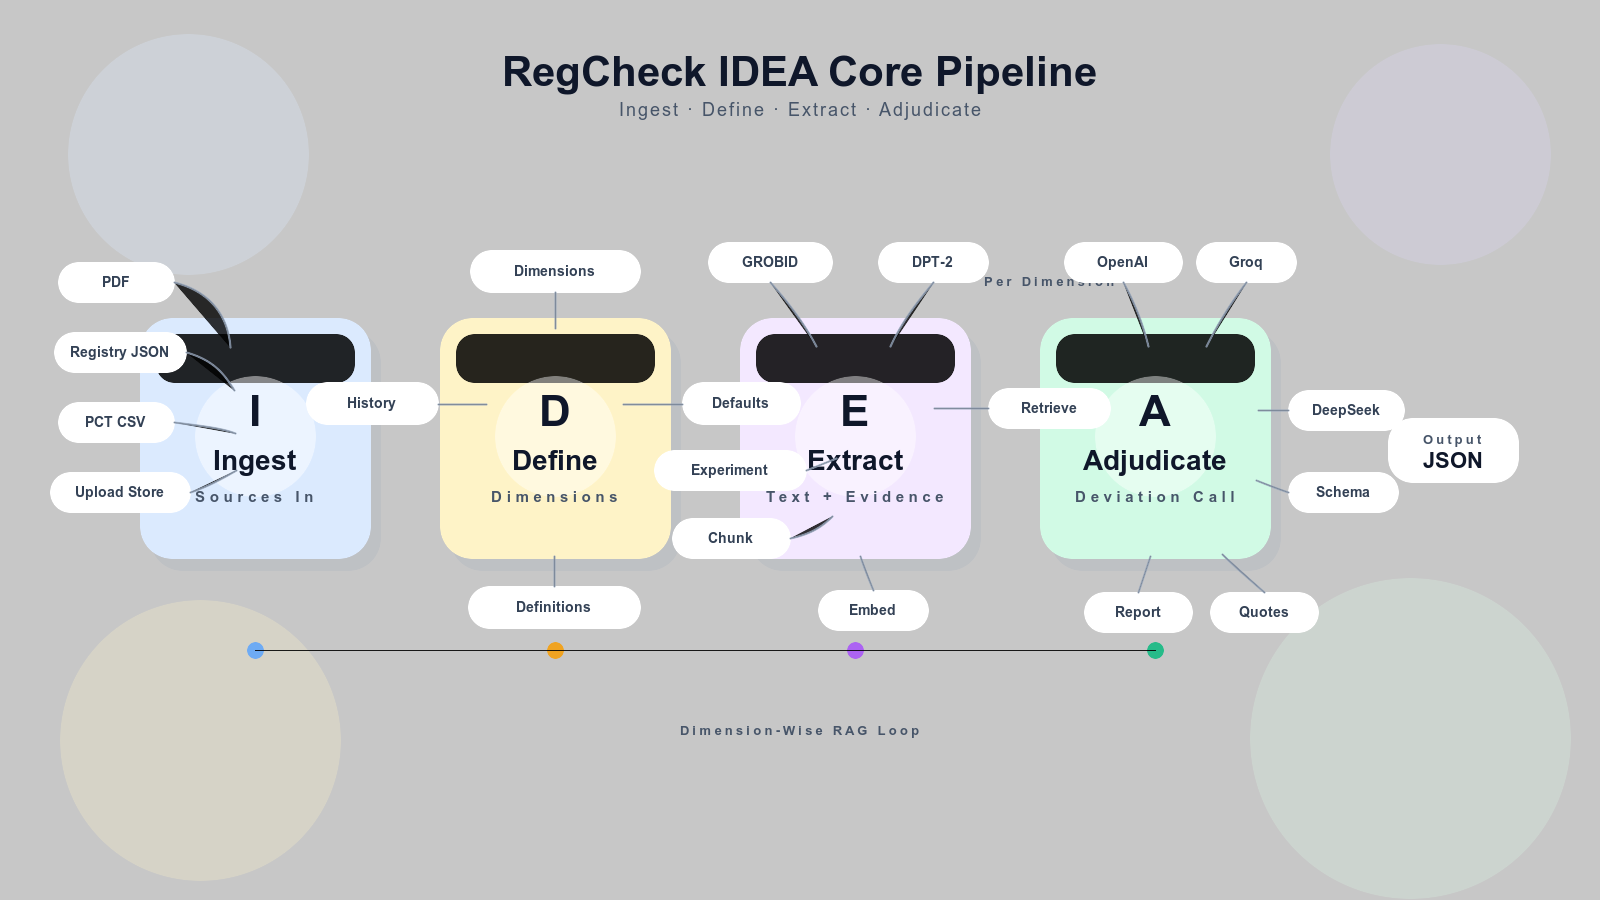
\includegraphics[width=0.9\linewidth]{regcheck_idea_core_pipeline.png}
  \caption{The IDEA framework: Ingest research materials in a structured,
  systematic manner; Define the dimensions along which to compare the research
  objects; Extract the text from each object which best relates to a given
  dimension of comparison; Adjudicate on whether the extracted text matches
  between research objects. Generative LLMs enter only at the final step.}
  \label{fig:idea}
\end{figure}

% ---------------------------------------------------------------------
\section{Dimensions as the Unit of Comparison}\label{sec:dimensions}
% [NEW SECTION] — assembled from v2 §7 (Non-prescriptive), §11, §4 stage 4,
% and §2 item 4; connective tissue is new, quoted material is verbatim.

The central representational choice in a Parity workflow is the Definition
step: the set of dimensions along which two artefacts are compared. It is not
the role of RegCheck to make determinations about which dimensions matter when
comparing a registration to a paper: this can vary by user, use case, and
field/discipline norms. There is no broad cross-discipline consensus, that we
know of, on the selection of dimensions which do or do not matter for study
registration. Nor is there an agreed-upon framework for what ultimately counts
as a deviation: different researchers disagree about what should be specified in
a registration, along what dimensions a registration should be compared to a
paper, and what ultimately counts as a deviation or not. The comparison basis
is, in other words, a normative choice---and the Definition step locates that
choice with the human user rather than leaving it implicit in a model's
behaviour. RegCheck therefore provides discipline-specific default dimensions
based on frequently examined features (e.g., sample size, primary outcomes),
organised into presets (for example, distinct dimension sets for psychology,
clinical/medical, economics, and preclinical/animal research), while also
providing free-text fields for users to add or redefine dimensions of their own.
Each preset contains default definitions that are specific to that field's
reporting conventions (for instance, clinical/medical defaults have a specific
focus on primary/secondary outcomes). Definitions are used both for text
extraction and for better-specified adjudication prompts.

Dimensions are also the unit of adjudication. By default, each comparison
dimension is adjudicated in its own call to the model, so that the output for
one dimension does not contaminate another. The rationale mirrors problem~4 of
\cref{sec:why-not-llm}: when multiple dimensions are evaluated in a single
generative pass, output is produced sequentially, errors propagate across
dimensions, and dimension-level accuracy can no longer be evaluated
independently. Per-dimension isolation makes each judgement independently
reproducible, independently verifiable by a human, and independently evaluable
in validation studies---the unit of comparison is thereby also the unit of
accountability.

Finally, dimensions are the unit of verdict. Each adjudication returns one of
three values---\emph{Deviation}, \emph{No deviation}, or \emph{Insufficient
evidence}---together with a brief supporting explanation that cites the
retrieved excerpts. The third value is a deliberate design commitment, not a
failure mode. Registries frequently lack fields that papers report (and vice
versa), and retrieval can fail to locate text that exists; a binary
consistent/inconsistent scheme would force both situations into a confident
verdict that the evidence does not support. Treating insufficient evidence as a
first-class outcome instead directs the human to the place where the tool's
knowledge ends---which, for a tool whose purpose is to support expert judgement
rather than replace it, is precisely the point at which the human should take
over. Mutual silence, on this scheme, is never counted as consistency.

% ---------------------------------------------------------------------
\section{RegCheck: An Instance of Parity}\label{sec:regcheck}

% [VERBATIM] v2 §4 opening ¶ + [NEW] pointer to appendix
RegCheck operationalises the four IDEA steps through a six-stage backend
pipeline. These additional stages reflect specific modifications to the
framework that serve to better facilitate the specific task of
registration--paper comparison. Stages 1--2 correspond primarily to
\textbf{Ingestion}, Stage 4 to \textbf{Definition}, Stage 3 together with the
retrieval component of Stage 5 correspond to \textbf{Extraction}, and the
judgement component of Stage 5 corresponds to \textbf{Adjudication}. Stage 6 is
an additional layer focused on reporting, which is not a core part of the IDEA
framework but is important to ensure the interpretability and ease of use of the
software. We summarise each stage here; \cref{app:pipeline} gives the full
stage-by-stage detail.

\begin{enumerate}
  % [COMPRESSED] v2 §4 stage 1
  \item \textbf{Ingestion.} The user specifies a registration and paper.
  Registrations can be provided by directly uploading a registration file, by
  referencing an entry in a public registry (e.g., ClinicalTrials.gov), or by
  linking to a hosted registration on the Open Science Framework; registrations
  obtained from registries or hosted repositories are handled through their
  structured-data interfaces rather than PDF parsing. Papers are accepted in a
  range of document formats; where a paper is supplied as a PDF, it is parsed
  using specialised document-layout models \citep{grobid_grobid_2025,
  huang_document_2025}, with an automatic fallback to alternative extractors
  when the selected primary parser cannot recover usable text.
  % [COMPRESSED] v2 §4 stage 2
  \item \textbf{Preparation.} Reference sections are stripped and layout is
  normalised. If the paper consists of multiple studies, irrelevant studies are
  removed, and only the general introduction, the relevant study, and general
  discussion are retained; follow-up extraction logic surfaces antecedent
  details described elsewhere in the paper (e.g., ``Our procedure was the same
  as the previous experiment'').
  % [COMPRESSED] v2 §4 stage 3
  \item \textbf{Embedding and indexing.} All content from both documents is
  split into short, sentence- and section-boundary-aware chunks with modest
  overlap, and embedded using a general-purpose semantic embedding model to
  support retrieval-augmented extraction. Because the embedding step is
  provider-neutral, the embedding model can be swapped---including for a locally
  or institution-hosted model---so that registration and paper text can be
  embedded without leaving a trusted environment.
  % [NEW] pointer — content covered in §4
  \item \textbf{Definition.} Users select a discipline preset or define their
  own dimensions, as described in \cref{sec:dimensions}.
  % [COMPRESSED] v2 §4 stage 5
  \item \textbf{Extraction and adjudication.} For each dimension, RegCheck
  retrieves the most relevant evidence excerpts from each source using dense
  embedding retrieval, complemented by a hybrid keyword search that promotes
  high-value chunks which a dimension's keywords match but which ranked just
  outside the similarity cut. The retrieved excerpts are sent to a user-selected
  LLM, which produces concise summaries of the dimension-relevant registration
  and paper content (referencing the excerpt IDs), and a deviation judgement
  from the same evidence, surfaced to the user as \texttt{Deviation},
  \texttt{No deviation}, or \texttt{Insufficient evidence} with a brief
  supporting explanation.
  % [COMPRESSED] v2 §4 stage 6
  \item \textbf{Reporting.} RegCheck renders an interactive, shareable report
  associated with a unique RegCheck report ID, with two views.
  \emph{Overview} presents, for each dimension, a colour-coded consistency
  judgement together with a rationale and summaries of the content from the
  study registration and paper; summaries and judgement texts directly cite
  specific excerpts from each document, allowing users to easily verify the
  claims made. \emph{Evidence} shows both source documents side-by-side with the
  relevant sections for a given dimension highlighted, so that users can conduct
  manual comparisons and verify the specific judgement provided by RegCheck
  (\cref{fig:report}). Reports can be exported as self-contained HTML files, and
  shared publicly or privately.
\end{enumerate}

\begin{figure}[t]
  \centering
  % TODO(jamie): use the current Overview screenshot asset from the arXiv build
  % (v2 Figure 3); Evidence-view screenshot (v2 Figure 4) moves to the appendix.
  \includegraphics[width=\linewidth]{regcheck-report-overview.png}
  \caption{The Overview section of a RegCheck report. The left panel specifies
  the dimension of interest, along with the associated judgement for this
  dimension; the central panel provides the rationale for this deviation
  judgement; the right panel provides overviews of the findings from the
  registration and paper. Here, one of the quotes specified in the report has
  been clicked, revealing the verbatim content of the quote to the user.}
  \label{fig:report}
\end{figure}

% ---------------------------------------------------------------------
\section{A Worked Example}\label{sec:worked-example}

% [VERBATIM] v2 §5 ¶1–¶2 (table pointer adjusted for the 6-row main-text table)
To make the workflow concrete, we walk through an illustrative example showing
how RegCheck can be used. The content of the trial registry/paper below is
hypothetical, but serves to show how RegCheck can provide a useful and
verifiable report that can facilitate registration--paper comparison.

Consider a randomised, placebo-controlled trial of a once-weekly drug, added to
standard care, for adults with type 2 diabetes. A reviewer has the manuscript
and the trial's public registry entry, and wants to check them against one
another using the RegCheck web application. Using the clinical-trial flow, the
reviewer enters the trial's ClinicalTrials.gov identifier and uploads the
manuscript, then opts for the clinical/medical dimension preset and runs the
comparison. RegCheck retrieves and structures the registration directly from the
registry, parses the manuscript, and for each dimension, chunks and embeds both
sources, retrieves the most relevant excerpts from each, summarises them, and
adjudicates whether the paper deviates from what was registered.
\Cref{tab:worked-example} shows six representative dimensions of the resulting
hypothetical report, spanning all three verdicts; the full eleven-dimension
report is reproduced in \cref{app:full-table}.

% [VERBATIM cells from v2 Table 1; 6 of 11 rows selected]
\begin{table}[t]
  \centering
  \caption{Six dimensions from an illustrative RegCheck report for the
  hypothetical type 2 diabetes trial (full report:
  \cref{app:full-table}). Registration excerpts are drawn from structured
  registry fields; evidence identifiers (e.g., \texttt{PREREG\_0011}) are the
  handles a reader clicks to jump to the highlighted excerpt in the source. All
  quotations are constructed for illustration.}
  \label{tab:worked-example}
  \footnotesize
  \begin{tabular}{@{}p{0.14\linewidth}p{0.27\linewidth}p{0.27\linewidth}p{0.24\linewidth}@{}}
    \toprule
    \textbf{Dimension} & \textbf{Registration (excerpt)} & \textbf{Paper
    (excerpt)} & \textbf{RegCheck verdict} \\
    \midrule
    Eligibility -- inclusion criteria &
    ``Adults aged 18--75 years with type 2 diabetes and a baseline HbA1c of
    7.0\%--10.0\%.'' [\texttt{PREREG\_0004}] &
    ``Eligible participants were adults aged 18--75 years with type 2 diabetes
    and a screening HbA1c of 7.0\%--10.0\%.'' [\texttt{PAPER\_0009}] &
    \textbf{No deviation.} The reported eligibility matches the registered
    criteria. \\
    \addlinespace[3pt]
    Eligibility -- exclusion criteria &
    ``Exclusion: estimated glomerular filtration rate below 30 mL/min.''
    [\texttt{PREREG\_0006}] &
    ``Patients with an estimated glomerular filtration rate below 45 mL/min
    were excluded.'' [\texttt{PAPER\_0011}] &
    \textbf{Deviation.} The renal-function exclusion threshold was tightened
    from 30 to 45 mL/min. \\
    \addlinespace[3pt]
    Sample size &
    ``Estimated enrolment: 300 participants, randomised 1:1.''
    [\texttt{PREREG\_0007}] &
    ``The trial was terminated early due to slow recruitment; 212 of a planned
    300 participants underwent randomisation.'' [\texttt{PAPER\_0014}] &
    \textbf{Deviation.} Enrolment fell short of the registered target and the
    trial was stopped early. \\
    \addlinespace[3pt]
    Outcomes -- primary &
    ``Primary outcome measure: change in HbA1c from baseline to Week 24.''
    [\texttt{PREREG\_0011}] &
    ``The primary endpoint was the proportion of participants achieving an
    HbA1c below 7.0\% at Week 24.'' [\texttt{PAPER\_0019}] &
    \textbf{Deviation.} The registered continuous primary outcome was replaced
    by a dichotomous responder endpoint and was not disclosed as a change. \\
    \addlinespace[3pt]
    Outcomes -- secondary &
    ``Secondary outcome measure: change in body weight from baseline to Week
    24.'' [\texttt{PREREG\_0021}] &
    No excerpt addressing body weight was retrieved from the manuscript text. &
    \textbf{Insufficient evidence.} The registered secondary outcome could not
    be located in the parsed manuscript. \\
    \addlinespace[3pt]
    Ethical approval -- number &
    The registry record does not contain an ethics approval number. &
    ``The study was approved under protocol number 2020-417.''
    [\texttt{PAPER\_0003}] &
    \textbf{Insufficient evidence.} The registry records no approval number, so
    the two cannot be compared. \\
    \bottomrule
  \end{tabular}
\end{table}

% [VERBATIM] v2 §5 ¶3–¶4 (five-dimension list retained; counts point to full table)
Two things can be immediately noted in this report. First, the presence of each
row immediately provides structure for the user in how to think about comparing
the registration and manuscript. Second, the distinct rows fall into categories
which demand one of three courses of action.

RegCheck states that the paper is consistent with the registration on five
dimensions of the full report (\textbf{Eligibility -- inclusion criteria}, the
\textbf{Intervention/treatment and control/placebo}, \textbf{Ethical approval --
committee}, \textbf{Date recruitment started}, and \textbf{Method of
randomisation and allocation}). Each of these is a row the reviewer can confirm
at a glance, following the evidence identifiers to the matching text in the
registry record and the manuscript. They additionally can scrutinise these
consistency judgements further by easily viewing the surrounding context of
these quotes around the extracted text to verify that RegCheck did not miss
anything important.

% [VERBATIM] v2 §5 deviations list
Three dimensions are flagged as ``deviations'', and they differ instructively in
their visibility:
\begin{enumerate}
  \item The \textbf{Outcomes -- primary} row exhibits a clear deviation, with
  the outcome registered as continuous (change in HbA1c) but reported in the
  paper as a dichotomous responder endpoint. Such outcome switching is at odds
  with CONSORT reporting standards, can alter the apparent strength of the
  findings, and is not disclosed as a change. At the same time, this subtle
  difference can be easy to miss in manual review: RegCheck facilitates this
  comparison by flagging it trivially.
  \item The \textbf{Eligibility -- exclusion criteria} row is an even subtler
  case, exhibiting a renal-function threshold changed from 30 to 45
  mL/min---yet again exactly the kind of small numeric change that is almost
  impossible to catch by eye but that can be trivially spotted and verified by
  RegCheck.
  \item The \textbf{Sample size} row catches a case of an early termination, as
  well as under-enrolment relative to the registered target. In each of these
  cases, RegCheck flags these issues because they are literal deviations, but
  RegCheck should not be used to outsource expert decision-making. Indeed, each
  of these departures may well be defensible with further expert scrutiny.
  However, they depart from what was registered, and are therefore flagged so
  that an expert can review them accordingly.
\end{enumerate}

% [VERBATIM] v2 §5 insufficient-evidence ¶ + [NEW] closing cross-reference
The remaining three rows of the full report return ``insufficient evidence''
for different reasons. For \textbf{Ethical approval -- number} and
\textbf{Ethical approval -- date}, the registry simply does not carry the
information, so there is nothing on the registration side to compare against.
RegCheck simply reports this absence of information directly and then moves on.
For \textbf{Outcomes -- secondary}, the registration may contain this
information, but the relevant text could not be located in the parsed
manuscript. Rather than assert that the outcome was dropped, RegCheck directs
the reviewer to confirm whether it is reported elsewhere (e.g., in a supplement
not provided to RegCheck). These rows are the three-valued verdict space of
\cref{sec:dimensions} doing its work: in neither case does the report
manufacture a confident verdict that the evidence cannot support.

% [VERBATIM] v2 §5 closing ¶
In each case, RegCheck has distilled a slow, full-document reading task to a
short, structured set of extractions and judgements that can be reviewed,
verified, or rejected in mere minutes. Indeed, this is precisely the use case of
RegCheck: to serve an orienting function to researchers and make a
registration--paper comparison manageable enough to actually perform in an
already cumbersome review workflow. The same applies to authors themselves, who
can run RegCheck on their own manuscripts before submission to catch and
disclose undetected deviations proactively. Importantly, RegCheck leaves the
substantive judgements (e.g., whether or not observed deviations are threatening
to the integrity of the research claims) where they belong: with the human
expert.

% ---------------------------------------------------------------------
\section{Validation}\label{sec:validation}
% [NEW section, replacing v2 §11; two retained v2 ¶s marked below]

% [VERBATIM] v2 §11 opening caveat (condensed)
RegCheck is not intended to replace human judgement. Users must apply their own
discretion when evaluating registration--paper consistency, and they should be
aware that RegCheck can make both false positive errors (flagging a deviation
where there is none) and false negative errors (missing a deviation that
exists). The evaluative question is therefore whether its extractions and
judgements agree with expert humans often enough to be useful.

% [NEW] companion validation summary
A companion validation study addresses this question directly in the
clinical-trials domain \citep{cummins_automating_2026}. Sixty-two trials
published in five high-impact general medical journals---each previously
audited manually by the COMPare project \citep{goldacre_compare_2019}---were
re-assessed using a RegCheck-based workflow for outcome identification and
misreporting detection. Against the expert audits, the workflow achieved 91.2\%
recall on outcome extraction and 83.6\% accuracy in classifying outcomes as
primary, secondary, or non-prespecified. Its detection of outcome misreporting
agreed with the human audit in 85.6\% of cases, rising to 94.8\% after
discrepancies between the automated and human assessments were adjudicated;
notably, a number of the initial disagreements were resolved in the automated
workflow's favour, indicating that it can catch discrepancies that manual
auditing missed. The average cost was \$5.94 (USD) per paper. We are explicit
about the scope of this evidence: it covers one discipline (clinical trials) and
one family of dimensions (outcomes). Parallel validations against human-coded
registration--paper comparisons in psychology, preclinical medicine, and
economics are ongoing.

% [VERBATIM] v2 §11 ¶2–¶3 (the evaluation-philosophy paragraphs, condensed)
Evaluating tools like RegCheck comes with challenges, because there is little
consensus on how to assess such performance in humans, let alone automated
tools: as discussed in \cref{sec:dimensions}, researchers disagree about what
should be specified in a registration and what ultimately counts as a deviation,
and some aspects of comparison are inherently ambiguous---whereas it can be
relatively straightforward to get agreement on a prespecified sample size, other
features (e.g., prespecified hypotheses or sufficiency of prespecified outcome
descriptions) can elicit more variation in the evaluations of humans. Put
simply: in many cases, establishing a ground truth among human comparators is
incredibly difficult. Rather than trying to evaluate RegCheck as software aimed
at approximating a known ground-truth value, we therefore treat and evaluate it
as an \emph{accompanying reviewer}: our core evaluation metric is the degree of
agreement with human comparators, and the establishment of relative
non-inferiority to observed human--human agreement. For us to consider RegCheck
sufficiently useful, it should, in general, show agreement with human raters to
at least the same extent as humans show agreement with one another. In cases of
disagreement, we also examine whether RegCheck is hallucinating or making
mistakes, or capturing legitimate details which humans tend to miss.

% ---------------------------------------------------------------------
\section{Limitations and Open Problems}\label{sec:limitations}
% [NEW section; assembled from v2 §7/§11/§12 with new honest limits]

The IDEA framework does not solve the normative problems it exposes. It does not
determine which dimensions matter---that remains a human choice, and defaults
encode our judgements of field conventions, not a consensus that does not
exist. Nor does it adjudicate severity: RegCheck flags literal departures from
what was registered, and whether a given departure threatens the integrity of
the claims is left, deliberately, with the human expert.

The framework's most distinctive output is also its least verifiable one. A
\emph{Deviation} or \emph{No deviation} verdict is supported by quotations the
user can check directly; an \emph{Insufficient evidence} verdict, by contrast,
can reflect a genuine absence in the source documents or a retrieval failure,
and the report cannot distinguish the two---the user must. This asymmetry is
inherent to any retrieval-based design, and improving the detectability of
retrieval misses is an open problem we consider a priority.

% [VERBATIM] v2 §7 discipline-aware caveat + §11 artificial-texts plan (one sentence)
We also recognise that RegCheck's accuracy and usefulness may vary across fields
and disciplines; for this reason, we are investigating variation in its accuracy
in a range of different domains. Beyond human-agreement studies, we additionally
plan to examine accuracy on artificially generated registration--paper pairs
with injected inconsistencies, which offers controlled ground truth at scale at
the cost of stylistic realism. Finally, the ongoing research agenda addresses
whether providing RegCheck to authors improves the quality of
registration--paper comparisons upon submission of papers to journals, and
whether it improves the efficiency and frequency of such comparisons.

% ---------------------------------------------------------------------
\section{Conclusion}\label{sec:conclusion}

% [VERBATIM] v2 §13 (final sentence extended with extensions from v2 §12)
Study registration promises to make the difference between planned and post hoc
decisions traceable, and to help readers calibrate their confidence in a result.
That promise is only realised when registrations are actually checked against
the papers they accompany. As empirical investigations demonstrate, this
checking is rarely done. One reason for this is that manual checking is slow,
repetitive, and easy to defer. One might argue that researchers can now simply
upload these documents to a large language model and prompt it to compare them:
however, this is necessarily unstandardised, both in terms of the specific
set-up provided to the LLM and the criteria along which the LLM may compare the
two materials.

RegCheck provides a systematic and structured approach to automated comparisons
of registrations and papers as a direct response to this gap. By using the
conceptual scaffolding of the IDEA framework, it decomposes the task into four
modular steps, enabling each step to be independently evaluated, and improved.
This also serves to delineate clearly where generative LLMs are and are not
required: their primary purpose is in the adjudication step, where synthesised
judgement is required.

The ultimate goal of RegCheck is to support researchers in engaging in an
otherwise rare scientific activity: comparing registrations to papers. Used in
this spirit, we believe RegCheck (and the Parity architecture behind it) can
help make consistency checking a routine part of the scientific writing and
review process in the social and medical sciences. We welcome engagement from
researchers, journals, and funders interested in using RegCheck in diverse
research areas, and we are developing extensions of the same architecture,
including the capacity to assess multiple papers at once for meta-scientific
research, and to assess consistency between study analysis code and
descriptions of planned analyses.

% ---------------------------------------------------------------------
\begin{ack}
% [VERBATIM] from v2 acknowledgements/funding (NeurIPS style: single ack env;
% remove for anonymous submission)
JC, BC, and ME are supported by a joint grant in the META-REP Priority Program
of the German Research Foundation (\#546323839) and the Swiss National Science
Foundation (\#100014E\_225145). We thank (in alphabetical order) Alison Avenell,
Anouk Bouma, Saloni Dattani, Matilda Fogato, Lukas Jung, Daniel Lakens,
Alexander Mainetti, Sabrina Norwood, Lars Schilling, Olmo van den Akker, Colby
Vorland, and Alexander Wuttke for providing valuable feedback on RegCheck's user
experience and output during the course of its development. RegCheck is open
source; code is available at
\url{https://github.com/JamieCummins/regcheck} under the GNU AGPL-3.0 licence.
\end{ack}

% ---------------------------------------------------------------------
% NEW bib keys needed in references.bib (all others exist from the arXiv build):
%   kaplan_likelihood_2015     — Kaplan & Irvin (2015), PLOS ONE 10(8):e0132382
%   higgins_recommendations_2026 — Higgins, Clarke, Elson & Cummins (2026), PsyArXiv
%   cummins_codebot_2026       — Cummins, Elson & DeVito (2026), github.com/JamieCummins/codebot
%   wilkinson_inspect-sr_2025  — Wilkinson et al. (2025), INSPECT-SR, medRxiv
%   cummins_automating_2026    — Cummins, Drysdale, Elson, Hussey, Goldacre &
%                                DeVito (2026), medRxiv 10.64898/2026.07.30.26358885
\bibliography{references}

% =====================================================================
\appendix
\newpage

\section{The RegCheck Pipeline in Full}\label{app:pipeline}
% [VERBATIM] v2 §4 stage detail not retained in the main text.

\paragraph{Ingestion.} Where a paper is supplied as a PDF, it can be parsed
using specialised document-layout models (such as GROBID
\citep{grobid_grobid_2025} or DPT-2 \citep{huang_document_2025}), with an
automatic fallback to alternative extractors when the selected primary parser
cannot recover usable text (e.g., from a scanned or atypically typeset
document). Registrations obtained from registries or hosted repositories are
handled through their structured-data interfaces rather than PDF parsing;
Open Science Framework links resolve to either a registration's structured
responses or an attached file. Critically, all of these parsing approaches are
engineered to ensure that relevant text content maintains its integrity and can
be properly handled in the subsequent steps.

\paragraph{Embedding and indexing.} All content from both documents is split
into chunks using a token-based, sentence-aware method. Chunks are kept
relatively short in length so that retrieved excerpts are tight, quotable, and
matched to the types of extractions that humans would typically provide. Chunk
boundaries are aligned to both sentence endings and section headings, so that
(for example) a methods detail is not embedded together with adjacent results
text. Consecutive chunks overlap by a modest amount, realised as whole trailing
sentences, so that important information straddling a boundary still appears
intact in at least one chunk. The exact chunk size and overlap are configurable
parameters via the RegCheck API and CLI. Local embeddings model usage is
supported for local use within the CLI.

\paragraph{Extraction and adjudication.} For each dimension, RegCheck forms a
single query from the dimension label plus its definition (user-provided or a
built-in default), embeds this query, and scores every registration and paper
chunk by cosine similarity. The number of excerpts retained scales with the
length of each source (so that a short, single-study text is not over-pruned)
and is complemented by a hybrid keyword search that promotes high-value chunks
which a dimension's keywords match but which ranked just outside the similarity
cut (e.g., a sentence which explicitly mentions a keyword like ``sample size''
or ``exclusion''). This process is the means by which RegCheck provides users
with direct quotes from the registration/paper for their own inspection.
RegCheck also uses these extracted quotes when constructing the adjudication
prompt, while additionally expanding each retrieved chunk into its neighbouring
chunks (a ``small-to-big'' approach) so that the model is also provided with
information about those chunks in-context. By default, each comparison dimension
is adjudicated in its own call, so that the output for one dimension does not
contaminate another.

\paragraph{Reporting.} The \emph{Evidence} view of the report is illustrated in
\cref{fig:evidence-view}. The left panel displays the quotes most relevant to
the specific dimension under examination from both the registration and paper.
The central and right panels provide renders of the text from the registration
and paper, respectively. When a quote of interest in the left panel is clicked,
the report automatically navigates in the registration or paper to the location
of the quote of interest.

\begin{figure}[h]
  \centering
  % TODO(jamie): v2 Figure 4 asset (Evidence view screenshot)
  \includegraphics[width=\linewidth]{regcheck-report-evidence.png}
  \caption{The Evidence section of a RegCheck report.}
  \label{fig:evidence-view}
\end{figure}

\section{Full Worked-Example Report}\label{app:full-table}
% [VERBATIM] v2 Table 1, all eleven rows.
\begin{table}[h]
  \centering
  \caption{The complete illustrative RegCheck report for the hypothetical type
  2 diabetes trial, showing all eleven dimensions of the clinical/medical
  preset. All quotations are constructed for illustration and are not derived
  from existing manuscripts or registrations.}
  \label{tab:full-example}
  \footnotesize
  \begin{tabular}{@{}p{0.14\linewidth}p{0.27\linewidth}p{0.27\linewidth}p{0.24\linewidth}@{}}
    \toprule
    \textbf{Dimension} & \textbf{Registration (excerpt)} & \textbf{Paper
    (excerpt)} & \textbf{RegCheck verdict} \\
    \midrule
    Eligibility -- inclusion criteria &
    ``Adults aged 18--75 years with type 2 diabetes and a baseline HbA1c of
    7.0\%--10.0\%.'' [\texttt{PREREG\_0004}] &
    ``Eligible participants were adults aged 18--75 years with type 2 diabetes
    and a screening HbA1c of 7.0\%--10.0\%.'' [\texttt{PAPER\_0009}] &
    \textbf{No deviation.} The reported eligibility matches the registered
    criteria. \\
    \addlinespace[3pt]
    Eligibility -- exclusion criteria &
    ``Exclusion: estimated glomerular filtration rate below 30 mL/min.''
    [\texttt{PREREG\_0006}] &
    ``Patients with an estimated glomerular filtration rate below 45 mL/min
    were excluded.'' [\texttt{PAPER\_0011}] &
    \textbf{Deviation.} The renal-function exclusion threshold was tightened
    from 30 to 45 mL/min. \\
    \addlinespace[3pt]
    Intervention/treatment and control/placebo &
    ``Experimental arm: 2 mg of the study drug subcutaneously once weekly;
    comparator: matching placebo.'' [\texttt{PREREG\_0009}] &
    ``Participants received 2 mg of the study drug or matching placebo
    subcutaneously once weekly, in addition to standard care.''
    [\texttt{PAPER\_0015}] &
    \textbf{No deviation.} Drug, dose, route, schedule, and comparator all
    match. \\
    \addlinespace[3pt]
    Ethical approval -- number &
    The registry record does not contain an ethics approval number. &
    ``The study was approved under protocol number 2020-417.''
    [\texttt{PAPER\_0003}] &
    \textbf{Insufficient evidence.} The registry records no approval number, so
    the two cannot be compared. \\
    \addlinespace[3pt]
    Ethical approval -- committee &
    ``Oversight: Institutional Review Board of the coordinating centre.''
    [\texttt{PREREG\_0002}] &
    ``The trial was approved by the Institutional Review Board of the
    coordinating centre.'' [\texttt{PAPER\_0004}] &
    \textbf{No deviation.} Both identify the same ethics committee. \\
    \addlinespace[3pt]
    Ethical approval -- date &
    No ethics approval date is recorded in the registry. &
    ``Ethical approval was obtained prior to enrolment.''
    [\texttt{PAPER\_0005}] &
    \textbf{Insufficient evidence.} Neither source states a specific approval
    date. \\
    \addlinespace[3pt]
    Sample size &
    ``Estimated enrolment: 300 participants, randomised 1:1.''
    [\texttt{PREREG\_0007}] &
    ``The trial was terminated early due to slow recruitment; 212 of a planned
    300 participants underwent randomisation.'' [\texttt{PAPER\_0014}] &
    \textbf{Deviation.} Enrolment fell short of the registered target and the
    trial was stopped early. \\
    \addlinespace[3pt]
    Date recruitment started &
    ``Study start date: March 2021.'' [\texttt{PREREG\_0008}] &
    ``Recruitment began in March 2021 and ended in November 2022.''
    [\texttt{PAPER\_0013}] &
    \textbf{No deviation.} The reported recruitment start matches the
    registered start date. \\
    \addlinespace[3pt]
    Outcomes -- primary &
    ``Primary outcome measure: change in HbA1c from baseline to Week 24.''
    [\texttt{PREREG\_0011}] &
    ``The primary endpoint was the proportion of participants achieving an
    HbA1c below 7.0\% at Week 24.'' [\texttt{PAPER\_0019}] &
    \textbf{Deviation.} The registered continuous primary outcome was replaced
    by a dichotomous responder endpoint and was not disclosed as a change. \\
    \addlinespace[3pt]
    Outcomes -- secondary &
    ``Secondary outcome measure: change in body weight from baseline to Week
    24.'' [\texttt{PREREG\_0021}] &
    No excerpt addressing body weight was retrieved from the manuscript text. &
    \textbf{Insufficient evidence.} The registered secondary outcome could not
    be located in the parsed manuscript. \\
    \addlinespace[3pt]
    Method of randomisation and allocation &
    ``Allocation: randomised; computer-generated sequence; 1:1; central
    allocation.'' [\texttt{PREREG\_0010}] &
    ``Participants were randomly assigned 1:1 using a computer-generated
    sequence with central allocation concealment.'' [\texttt{PAPER\_0017}] &
    \textbf{No deviation.} The described randomisation and allocation match the
    registration. \\
    \bottomrule
  \end{tabular}
\end{table}

\section{Use Cases}\label{app:use-cases}
% [VERBATIM] v2 §6
The most obvious use case for RegCheck is for editors and reviewers who are
assessing a manuscript where one or more studies were registered (where they
have permission to share and upload those materials; see
\cref{app:privacy}). Similarly, research synthesists might use it when assessing
the trustworthiness of studies included in a systematic review or meta-analysis,
given the growing emphasis on such checks from organisations such as Cochrane
\citep{wilkinson_inspect-sr_2025}. Indeed, INSPECT-SR (the Cochrane-endorsed
checklist for conducting trustworthiness checks in systematic reviews;
\citealp{wilkinson_inspect-sr_2025}) focuses a portion of its checks on
registration--trial consistency, and RegCheck will be included as an endorsed
tool in the next iteration of INSPECT-SR. Of course, RegCheck is also useful for
authors who want to check their own manuscripts for any deviations they should
report (e.g., RegCheck could help to spot registration deviations that might be
missing in a registration deviation table, like the one suggested by
\citealp{willroth_best_2024}). Regardless of whether the user is using RegCheck
to assess their own paper or someone else's, the process is the same.

\section{Design Principles and Philosophy}\label{app:design}
% [VERBATIM] v2 §7
\begin{itemize}
  \item \textbf{Pragmatism.} RegCheck is a software tool which provides a
  standardised framework for checking registrations against papers, with the
  goal of increasing the frequency of registration--paper comparisons (which is
  not done regularly).
  \item \textbf{Human-in-the-loop.} RegCheck facilitates human experts; it does
  not replace them. The system highlights candidate discrepancies, and also
  provides indicative LLM-based judgements, but it is not intended to substitute
  human expertise.
  \item \textbf{Non-prescriptive.} It is not the role of RegCheck to make
  determinations about which dimensions matter when comparing a registration to
  a paper: this can vary by user, use case, and field/discipline norms. There is
  no broad cross-discipline consensus, that we know of, on the selection of
  dimensions which do or do not matter for study registration. RegCheck
  therefore provides discipline-specific default dimensions based on frequently
  examined features (e.g., sample size, primary outcomes), spanning a range of
  fields, while also providing free-text fields for users to add or redefine
  dimensions of their own.
  \item \textbf{Discipline-agnostic and discipline-aware.} Although it has
  origins in psychological research, RegCheck is an abstract workflow aimed at
  being useful for researchers across a range of scientific disciplines, and
  supports distinct comparison flows for different registration types (for
  example, preregistrations, clinical-trial registrations, and
  preclinical/animal-study registrations). At the same time, we recognise that
  RegCheck's accuracy and usefulness may vary across fields and disciplines;
  for this reason, we are investigating variation in its accuracy in a range of
  different domains.
  \item \textbf{Modular separation of roles.} Because RegCheck is built as a
  specific instance of Parity's research artefact comparison, it explicitly
  separates document ingestion, human definition of dimensions,
  similarity-based evidence extraction, and model-based adjudication. This
  makes the system easier to audit, evaluate, and extend, and it clarifies that
  errors in one part of the workflow need not be attributed wholesale to ``the
  LLM''. RegCheck's modularisation also enables it to keep pace with the rapid
  release of new models and tools in this fast-evolving space. By structuring
  the workflow through the IDEA framework, individual components can be readily
  updated or replaced as improved models become available.
\end{itemize}

\section{Privacy, Confidentiality, Accounts, and Sharing}\label{app:privacy}
% [VERBATIM] v2 §8
To create the persistent, shareable report page, RegCheck stores the artefacts
used to create the report: namely, the text excerpts and quotes extracted for
each dimension, the rendered document pages that are shown in the Evidence view,
and a copy of the source documents (i.e., registration/paper) used to render
that view. For reports generated anonymously (i.e., by a user who is not logged
in), these artefacts are retained only for a limited period (approximately 7
days) and are then deleted automatically. For signed-in users, RegCheck stores
generated reports indefinitely, but also offers users the ability to delete
their generated reports at any time.

RegCheck provides users with the option to decide which generative LLM is used
in the creation of the RegCheck report. Some of these models are open-weights
models which are hosted on third-party inference API providers (e.g., the Groq
service). Others are closed-source models which are hosted by those commercially
invested in that model (e.g., OpenAI serves its own models). LLM providers
typically state in their documentation that text served to its models via its
API service is not retained nor used for training. However, we of course have no
control over the enforcement of, and adherence to, these privacy policies, nor
do we have the capacity to know whether such policies may change in the future.
We therefore provide the open-weights models as alternative options, which are
hosted by third-party providers who are not commercially invested in the
development of the models they host. RegCheck can also be run fully locally,
either via its CLI, or by forking the open-source repository and running the
service locally.

Usage of RegCheck should be constrained by the same standards of confidentiality
and privacy around academic materials that apply in any other professional
context. In other words: just as one should not share confidential materials
with unauthorised colleagues, one should not upload such materials to RegCheck.

% [VERBATIM] v2 §9
RegCheck can be used entirely anonymously, but users may create an account
(using a supported identity provider, such as Google or ORCID) to use a small
set of collaboration features. Signed-in users can name and retain the reports
they generate, browse them from a personal dashboard, and control who can view
each report. Report visibility is two-tiered: a report can be made public, so
that anyone with its RegCheck ID link can open it, or kept private, in which
case access is restricted to an explicit allow-list of collaborators (with a
RegCheck account) identified by verified email address or ORCID iD. This makes
it possible, for example, for an editor to share a confidential comparison only
with the assigned reviewers. For programmatic and higher-volume use, RegCheck
also exposes an HTTP API authenticated with per-user API keys, mirroring the
comparison capabilities of the web app so that comparisons can be scripted or
integrated into editorial and meta-research pipelines.

\section{Running RegCheck Online and Locally}\label{app:local}
% [VERBATIM] v2 §10
RegCheck is freely available to use. Its point-and-click web application is
available at \url{https://regcheck.app}, and the open-source code, which can be
run locally at one's own cost, is available on GitHub. The cost of running a
comparison varies with the size of the registration and paper and with the
selected model; for users of the public web application, these costs are
currently covered by our research group, and use is free.

Beyond its web app, RegCheck comes with a headless command-line interface (CLI)
for running comparisons entirely locally without any hosted infrastructure. The
CLI covers the same comparison flows as the web app, takes comparison dimensions
either from the built-in discipline presets or from a user-supplied file, and
can be used with either hosted or fully local model providers. This makes it a
natural path for privacy-sensitive use: paired with a local embedding endpoint
and a locally hosted language model, an entire comparison can be run with no
document or text leaving the user's environment. The CLI can write the same
interactive report as a single self-contained offline HTML file, so that a
report can be archived or shared as a file rather than as a link. The CLI also
offers an additional feature, \emph{consensus mode}, that re-runs the
adjudication step several times per dimension. The final judgement reported is
the verdict representing the plurality of these calls. This offers protection
against the stochasticity of LLM outputs, which can be particularly problematic
for smaller models that will likely be used in local workflows.

\end{document}
